\begin{tikzpicture}
    \begin{scope}
        \clip (-2,-2) rectangle  + (4,4);
        %\draw [very thin, green, fill=yellow]  (-6,-4) rectangle (12,8);
        \node[inner sep=0pt] (russell) at (-8.1,0)
            {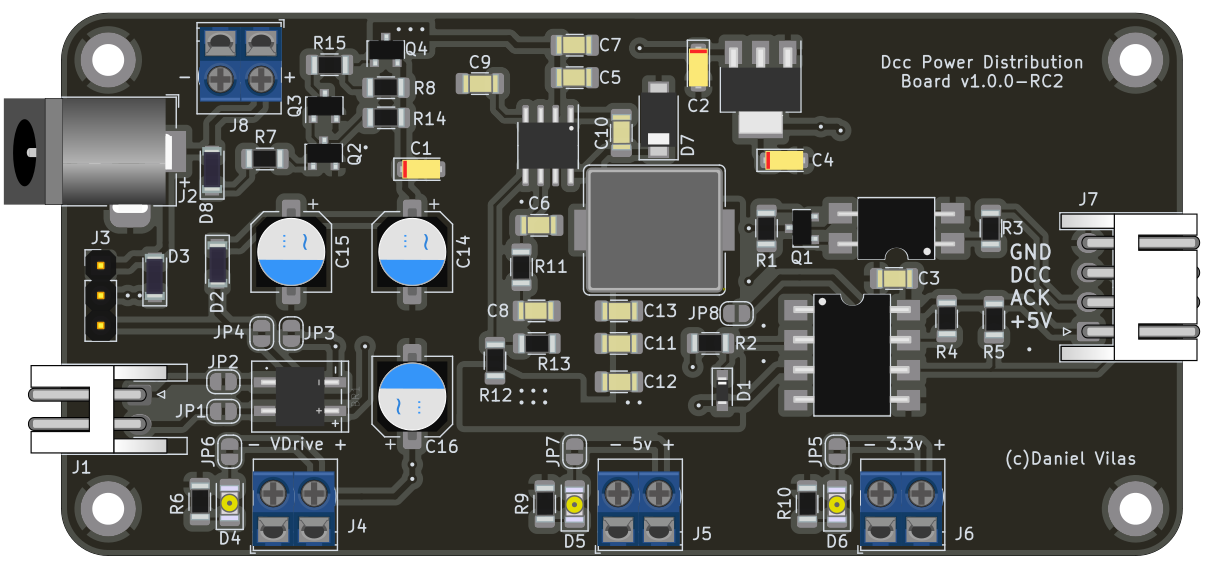
\includegraphics[scale=2]{images/front.png}};
        %\draw [very thin, green]  (-7,-3) grid (6,4);
    \end{scope}
    %\draw [very thin, green] (-3,-2) grid (3,2);
    \draw [color=yellow,line width=2pt](-1.6,-0.9) rectangle + (1.6,1.8);
    
    \node[right] at (4,1) {GND: Ref 0V};
    \node[right] at (4,0.33) {DCC-TTL: Salida Señal DCC};
    \node[right] at (4,-0.33) {ACK: Entrada Señal ACK};
    \node[right] at (4,-1) {+5V: Entrada/Salida Ref TTL};
    
    \draw [color=black, line width=3pt,cap=round] (2.0,0.75) -- (4,1);
    \draw [color=blue, line width=3pt,cap=round] (2,0.25) -- (4,0.33);
    \draw [color=orange, line width=3pt,cap=round] (2,-0.25) -- (4,-0.33);
    \draw [color=red, line width=3pt,cap=round] (2.0,-0.75) -- (4,-1);
\end{tikzpicture}